\chapterimage{contrasena-codigo-binario.jpg}
\chapter{Seguridad de datos - Criptografía}
\vspace{95px}
\begin{flushright}
    \textit{ }
\end{flushright}
%capitulo 7
%Seguridad de datos
 %       \begin{itemize}
  %          \item Criptografía \textbf{OK}
   %         \item Forense digital
    %        \item Integridad de datos y atenticación
     %       \item control de accceso
      %      \item protocolos de comunicación segura
       %     \item \gls{Criptoanálisis} \textbf{OK}
        %    \item privacidad de datos
         %   \item seguridad en almacenamiento de información
        %\end{itemize}
 
%tipos (simétrica, asimétrica, hashing), 
%aplicaciones (encriptación, firmas digitales, firma digital, SSL/TLS, Blockchain). 



\section{Una breve historia de la criptografía}
La criptografía es donde la ingeniería de seguridad se encuentra con las matemáticas. 
La criptografía se ha usado para proteger información por al menos 4000 años. La Estenografía fue el primer método. Ejemplo de mensajes en cuero cabelludo de personas que cuando arribaban a puerto eran rapadas para poder descubrir el mensaje.  




El cifrado de sustitución más famoso es el cifrado Cesar, en el cual cada letra en el alfabeto ingles es movido un número fijo de posiciones, que cuando al llegar a la Z vuelve a la A. Dado que se usa el alfabeto, el espacio de llaves es 25.
%
Dicen que Julio Cesar cifraba sus mensajes escribiendo una 'D' en vez de 'A', una 'E' en vez de 'B', y así. Luego Augusto Cesar utilizó una 'C' para la 'A' y una 'D' para la 'B', y así. 

Otro tipo de cifrado son los de transposición.
Cifradores de transposición reordenan los caracteres o bits de datos. Por ejemplo al escribir un mensaje de 9 caracteres en una matriz de cuatro columnas, avanzando fila por fila, hará que al leer la info de columna a columna el mensaje en texto plano esté cifrado. Esto implica que la llave de cifrado es {1,2,3,4}. Un cifrado de transposición simplemente reordena la información que debe ser reensamblada luego. 



En la primera y segunda guerra, la comunicación por radio era primordial para las comunicaciones entre las tropas, donde la criptogragía jugó un papel importante para proteger las comunicaciones. Existen casos interesantes de buscar donde estos `àlgoritmos'' fueron rotos, tales como: Cifrado purpura de los japoneses y el enigma de Alemania.  

La invención de los computadores hace posible el cifrado. Computadores digitales pueden realizar operaciones en segundos. 



La criptografía permite potencialmente abordar cuatro metas básicas: confidencialidad, integridad, autenticación y no repudiación. 


\begin{itemize}
    \item \textbf{Confidencialidad}: asegurado por un mensaje encriptado, mientras no hubiera un atacante que tenga la llave y pueda resolverla
     Además la criptografía puede reforzar la integridad con valores hashes o checksums, que son un calculo de una vía que lleva a un resultado que es usualmente más pequeño que el mensaje riginal y es difícil de duplicar. 
    \begin{itemize}
    \item checksum del número 56-9-88883432 podría ser la suma de sus dígitos = 64. Aunque sepamos el checksum no podemos recrear el número, pero si podemos decir si el teléfono que llegó calza con el checksum. 
    \item si recibimos una alteración del número 56-9-88483432 el checksum sería 60.
    \item No es un método seguro pues el atacante podría buscar un número que de igual checksum. 
    \item ayudan más a detectar errores accidentales que maliciosos. 
    \end{itemize}
    \item \textbf{autenticación}: provee la identidad al remitente si ambos coinciden e intercambian elementos. 
    \begin{itemize}
        \item método tradicional password
        \item criptografía de clave simétrica igual problema que una password - pues puede atrapar la llave tal como puede atrapar la password. 
    \end{itemize}
    \item \textbf{no repudiación}:antes,  no era posible con la criptografía de llave simétrica  probar que una parte haya originado un mensaje, porque cualquier persona con acceso a la llave compartida podría originar un mensaje. Por lo tanto, antes de la disponibilidad de la criptografía de llave asimétrica, no se podía probar quién escribió un mensaje.
    
\end{itemize}






\section{Encriptar/Cifrar}
Encriptar es 
\begin{itemize}
    \item Acto o arte de escribir en caracteres secretos
    \item codificar datos de manera que sólo puedan ser decodificado por individuos específicos
    \item arte de transformar un mensaje leible en una forma que es sólo leible por usuarios autorizados
\end{itemize}
La criptografía se compone de algoritmos o cifrados, usados para encriptar y desincriptar datos, que son utilizados de manera colectiva en un criptosistema. La mayoría de los cifradores toman data en texto plano y usan una o más llaves (es decir un string de números o caracteres conocidos solo para el que envía o el que recibe) para transformar el texto plano en un mensaje secreto - llamado textocifrado. 
\begin{tcolorbox}[colback=gray!5!white,colframe=orange!60!gray,title=¿es seguro?]
la seguridad del sistema de encriptado depende de lo secreto de las llaves en vez de lo secreto del cifrado. Es más robusto cuando por fuerza bruta es casi imposible de saber cual es la key.  
\end{tcolorbox}



La encriptación y desencriptación tradicional utiliza procesos matemáticos conocidos llamados algoritmos  (procesos que pueden producir la misma salida con la misma entrada) para realizar funciones. 
El algoritmo que específicamente encripta y desencripta información se llama cifrador. 
Por ejemplo: Algoritmo que adiciona $X$ a cada valor para encriptar, debería tener que restarle $X$ a cada valor para desencriptar. 
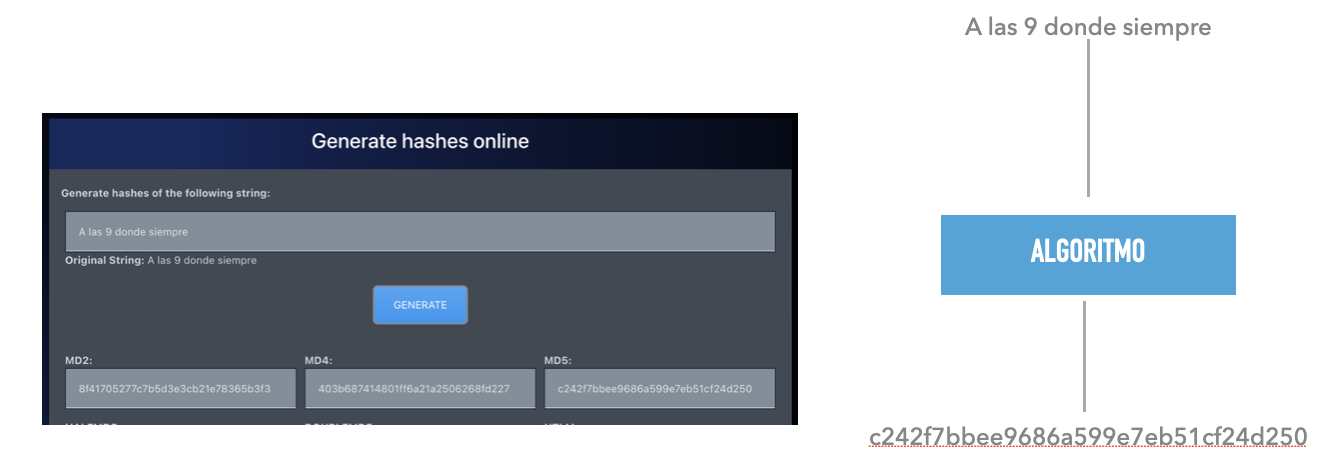
\includegraphics[scale=0.5]{imgs/sistemaencriptador.png}

\begin{tcolorbox}[colback=gray!5!white,colframe=orange!60!gray,title= Todo algoritmo encriptador tiene un desencriptador?]
Algunos algoritmos encriptadores son de una vía. Su uso: generar hashs. Funciones de hashing son últiles para proteger datos de cambios no autorizados. 
\end{tcolorbox}

\begin{tcolorbox}[colback=gray!5!white,colframe=orange!60!gray,title= Todos requieren key?]
No todos los cifradores requieren llave. Algunos tipos nuevos de algoritmos encriptadores derivan sus llaves de otra información, lo cual es un enfoque similar a control de acceso que usa entradas en vez de passwords. %Por ejemplo:\textbf{IBE - Identity-based Encryption} - usa identidad para derivar una llave y \textbf{ABE: Attribute-based encryption} usa atributos descriptivos para encriptar y desincriptar datos.
\end{tcolorbox} 

La mayoría de los cifrados de encriptación requieren texto plano y al menos una llave criptográfica, que es usada por el cifrador para variar sus salidas de manera de proteger de otros que utilicen el mismo cifrador. Al cambiar la llave, se cambia la salida de la función criptográfica, incluso si el texto plano sigue igual. 


Dos categorías generales de cifradores:
\begin{itemize}
    \item Esos que usan la misma llave para encriptar y desincriptar son \textbf{cifrados de llave privada simétrica}
     \item Esos que usan  llave diferente para encriptar y desincriptar son \textbf{cifrados de llave pública simétrica}
\end{itemize}
\begin{tcolorbox}[colback=gray!5!white,colframe=orange!60!gray,title= llaves débiles y ataques]
Las \textbf{técnicas de estiramiento de llave} pueden hacer que una llave débil sea más resistente a los ataques de fuerza bruta. Para lograr esto, una función de estiramiento de llave toma una llave (generalmente débil) como entrada y genera una llave mejorada que puede resistir un ataque más decidido.
\end{tcolorbox}


En el siglo 21 la fuerza de la criptografía se basa en el tiempo en que se puede romper los cifradores. Sin embargo, la criptografía cuántica, pone en riesgo aquello. 

Algoritmos cuánticos existentes tales como Shor y Grover, son capaces de romper algoritmos criptográficos simétricos y asimétricos dado un computador cuántico suficientemente grande. 



En 2029 se espera de Google un computador cuántico de 1 millón de qbits - teóricamente le tomará 7 años para romper la Blockchain usada en Bitcoin actualmente. 


Ahora bien, el uso popular de criptografía cuántica permitirá intercambiar llaves en una manera más segura que los computadores actuales. 


Con suficiente tiempo y recurso un atacante puede eventualmente desinscriptar cualquier texto cifrado. Por lo tanto la meta de la criptografía no es hacer el texto cifrado  desincriptable sino que el costo y el tiempo requerido sea tan alto sin la llave que exceda el valor de la información protegida. 
\begin{tcolorbox}[colback=gray!5!white,colframe=orange!60!gray,title= ataques]
Sin ningún conocimiento de la llave, un atacante con acceso a un mensaje encriptado y al cifrador desincriptador puede hacer un ataque de fuerza bruta: podría tratar todas las posibles llaves para decodificar un mensaje. Si el espacio de llaves es suficientemente grande, el costo de un ataque por fuerza bruta es muy alto. Si el cifrado no tiene debilidades matemáticas, entonces un espacio de llaves más grande usualmente significa más seguridad. 
\end{tcolorbox}


Para determinar la debilidad matemática en cifrado, expertos alrededor del mundo usan cifrados de código abierto para que sea extensamente analizado, y de haberlas, reportar las debilidades que podrían afectar la fuerza del cifrado. El Data Encryption Standard (DES) publicado en 1977 como Estandar Federal para el procesamiento de Información ha sido el cifrado más analizado en la historia. Su espacio de llaves posibles es de 72 cuadrillones sin encontrar hasta ahora ninguna debilidad matemática. 



\begin{tcolorbox}[colback=gray!5!white,colframe=red!60!gray,title= ADVERTENCIA]
Siempre usar algoritmos criptográficos probados en vez de escribir los propios. La historia muestra que los algoritmos criptográficos desarrollados de manera privada son más débiles que algoritmos abiertos. Por lo tanto, no es substituible que expertos alrededor del mundo validen rigurosamente la fuerza del algoritmo.
\end{tcolorbox}

\section{Rol de la criptografía en la seguridad de la información}


\begin{tcolorbox}[colback=gray!5!white,colframe=orange!60!gray,title= Usos]
Protegener los datos en tránsito (intercambios típicamente por una conexión de red)y proteger los datos ``en descanso'' (datos en almacenamiento y cualquier dato en memoria).
\end{tcolorbox}

\begin{tcolorbox}[colback=gray!5!white,colframe=orange!60!gray,title= Enfoques para asegurar las comunicaciones]
encriptar cada mensaje antes de enviarlo, lo que requiere un software para encriptar y desencriptar mensajes separado de la función de comunicaciones dejando que encripte los mensajes a medida que son transmitidos o recibidos (ocurriendo el encriptado en la capa de transporte).  
\end{tcolorbox}

\begin{tcolorbox}[colback=gray!5!white,colframe=orange!60!gray,title= SSL/TLSs]
Protocolos de encriptación de la capa de transporte son: Secure sockets kayer (ssl) y transport layer security (tls), que son comunmente usados para crear conexiones seguras entre servidores web y browsers. También con secure shell que es usado para setear las sesiones de login segura a sersvidores remotos.  
\end{tcolorbox}

 





\section{Criptografía simétrica y asimétrica}
\subsection{Criptografía asimétrica}
Diffie y Hellman de Stanford en 1976 publicaron un paper que introduce el concepto de \textbf{criptografía de llave asimétrica}. Introdujeron un método para intercambiar llaves simétricas usando técnicas asimétricas. \textbf{Uso más común:} asegurar comunicaciones entre dos partes, donde hoy, las aplicaciones de red establecen sesiones. 

Una manera de proteger los mensajes intercambiados es crear dos llaves únicas, llamadas llaves de sesión. Usando el algoritmo Dffie-Hellman, tanto el enviador como el receptor, usan encriptación asimétrica para asegurar el intercambio de las llaves simétricas. Luego de eso, cada uno puede usar una encriptación simétrica para encriptar y desencriptar la data. Bueno, debido a que los algoritmos de encriptación simétrica siempre son más rápidos que los asimétricos y tienen garantías de seguridad similar. Protocolos que consideran la base este algoritmo: 
\begin{itemize}
    \item Diffie-Hellman Ephemeral - usa aritmética modular para generar llaves
    \item Elliptic Curve DHE - usa curvas algebraicas para generar llaves
    
\end{itemize}
Ambos usan llaves efímeras (se crean en cada sesión). Dado que cada nuevo intercambio de llaves usa llaves asimétricas nuevas, cada proceso de setup de sesión es único. Por lo tanto, si las llaves de la sesión previa están comprometidas por un atacante, entonces, ninguna de las sesiones previas están en riesgo (perfect forward secrecy).

Cifrdo de llave simétrica usa la misma llave para encriptar el texto plano en cifrado como para desencriptarlo de vuelta a texto plano. Requiere que ambas partes intercambien primero la llave para poder comunicarse de manera segura. A esto se le denomina el problema del huevo y la gallina.

Si Alice y Bob acuerdan crear una sesión segura para comunicarse, utilizando DES. DES es público por tanto usando un software DES, Alice envía a Bob el mensaje de utilizar XXX como la llave. Bob está de acuerdo y le envía a Alice un mensaje encriptado usando esa llave. Para mitigar este problema la llave debe intercambiarse en otro canal.


Diffie y Hellman apuntan que el costo y retardo impuesto por el problema de distribución clave es la mayor barrera a la transferencia de comunicaciones de negocio para grandes redes de teleprocesamiento. 

Cifrados de llave asimétrica tiene cuatro propiedades:
\begin{itemize}
    \item dos algoritmos asociados que son inversos del otro: 
\end{itemize}





\newpage
\section{Hash}
\subsection{¿Qué es una función hash?}
Ya vimos en el capítulo de repaso que son las funciones hash. 
%
Una función hash toma algunos datos de entrada de cualquier tamaño y crea un resumen de esos datos. La salida tiene un tamaño fijo. Es difícil predecir cuál será la salida para cualquier entrada y viceversa. Los buenos algoritmos hash serán (relativamente) rápidos de calcular y lentos de revertir (pasar de la salida y determinar la entrada). Cualquier pequeño cambio en los datos de entrada (incluso un solo bit) debería causar un gran cambio en la salida.
%
La salida de una función hash normalmente son bytes sin formato, que luego se codifican. Las codificaciones comunes para esto son base 64 o hexadecimal. Son  diferentes del cifrado. No hay llave, y se supone que es imposible (o muy, muy difícil) volver de la salida a partir de la entrada.

También vimos que una colisión hash es cuando 2 entradas diferentes dan la misma salida. Las funciones hash están diseñadas para evitar esto lo mejor que pueden, especialmente para poder diseñar (crear intencionalmente) una colisión. Debido al efecto casillero, las colisiones no son evitables. El efecto de casillero es básicamente, hay un número determinado de valores de salida diferentes para la función hash, pero puede darle cualquier tamaño de entrada. Como hay más entradas que salidas, algunas de las entradas deben dar la misma salida. Si tiene 128 palomas y 96 casilleros, algunas de las palomas tendrán que compartir.
\textbf{Un hash no se considera criptográficamente seguro si dos archivos tienen el mismo valor hash o resumen.}


\textbf{Si tiene una salida hash de 8 bits, ¿cuántos hash posibles hay? 256
}

\subsection{Algoritmos de Hash más comunes}

Los siguientes son algunos de los algoritmos hash más comunes: 
\begin{itemize}
    \item MD5 (Message Digest, definido por  RFC 1321 ) : fue diseñado por Ron Rivest en 1992 y es una función hash criptográfica ampliamente utilizada con un valor hash de 128 bits. Los hashes MD5 NO se consideran criptográficamente seguros. En 2011, el IETF publicó RFC 6151, "Consideraciones de seguridad actualizadas para los algoritmos MD5 Message-Digest y HMAC-MD5", que mencionaba una serie de ataques contra hashes MD5
\item SHA-1 (Algoritmo Hash Seguro 1, definido por  RFC 3174 ) :  fue inventado por la Agencia de Seguridad Nacional de los Estados Unidos en 1995.  Cuando los datos se envían al algoritmo Hashing SHA-1, SHA-1 toma una entrada y produce un hash de 160 bits. cadena de valor como un número hexadecimal de 40 dígitos. El NIST desaprobó el uso de SHA-1 en 2011 y prohibió su uso para firmas digitales a finales de 2013 por ser susceptible a ataques de fuerza bruta. En cambio, NIST recomienda migrar de SHA-1 a algoritmos hash más potentes de las familias SHA-2 y SHA-3.
\item El SHA-2 (Secure Hash Algorithm 2) - Algoritmo de hash SHA-2 fue diseñado por el Instituto Nacional de Estándares y Tecnología ( NIST ) y la Agencia de Seguridad Nacional (NSA) en 2001 para reemplazar SHA-1. SHA-2 tiene muchas variantes y posiblemente la más común sea SHA-256. El algoritmo SHA-256 devuelve un valor hash de 256 bits como un número hexadecimal de 64 dígitos. 

\end{itemize}




\begin{tcolorbox}[colback=gray!5!white,colframe=orange!60!gray,title=¿Usamos hashing para encriptar llaves?] 
\textbf{MD5} y \textbf{SHA1} han sido atacados y se han vuelto técnicamente inseguros debido a colisiones de hash de ingeniería. Sin embargo, ningún ataque ha provocado una colisión en ambos algoritmos al mismo tiempo, por lo que si usa el hash \textbf{MD5} Y el hash SHA1 para comparar, verá que son diferentes. El ejemplo de colisión \textbf{MD5} está disponible en  \url{https://www.mscs.dal.ca/~selinger/md5collision/} y los detalles de la colisión SHA1 están disponibles en  \url{https://shattered.io/}. Debido a esto, no debe confiar en ninguno de los algoritmos para cifrar contraseñas o datos.\\
La función hash \textbf{MD5} produce una salida de 128 bits, que equivale a 16 bytes. Por lo tanto, el tamaño de salida en bytes de la función hash \textbf{MD5} es 16 bytes. Es importante tener en cuenta que \textbf{MD5} se considera obsoleto en la actualidad debido a vulnerabilidades conocidas en su diseño, y se recomienda utilizar algoritmos de hash más seguros, como \textbf{SHA-256} o \textbf{SHA-3}, para aplicaciones críticas de seguridad.\\
\end{tcolorbox}







\subsection{Usos para hash}
Hashing se utiliza para verificar la integridad de los datos, o para verificar contraseñas. La mayoría de las aplicaciones web necesitan verificar la contraseña de un usuario en algún momento. Almacenar estas contraseñas en texto sin formato sería malo. Bastantes violaciones de datos han filtrado contraseñas de texto sin formato. Casos:
\begin{itemize}
    
\item  empresa que hizo widgets para MySpace. Almacenaron sus contraseñas en texto sin formato y la empresa tuvo una violación de datos. El archivo ``rockyou.txt'' en Kali como una lista de palabras de contraseña contiene más de 14 millones de contraseñas 

\item Adobe: Las contraseñas estaban encriptadas, en lugar de cifradas y el encriptado que se utilizó no era seguro. Esto significaba que el texto sin formato podía recuperarse con relativa rapidez.  \footnote{\url{https://nakedsecurity.sophos.com/2013/11/04/anatomy-of-a-password-disaster-adobes-giant-sized-cryptographic-blunder/}}

\item Linkedin usó SHA1 para la verificación de contraseñas, que es bastante rápido de calcular usando GPU. 

\end{itemize}

\noindent Las contraseñas no deben encriptarse, ya que la llave debe almacenarse en algún lugar. Si alguien obtiene la llave, simplemente puede descifrar las contraseñas.
%
Por tanto, en vez de almacenar la contraseña, solo almacene el hash de la contraseña.  Esto significa que nunca tendrá que almacenar la contraseña del usuario, y si su base de datos se filtró, un atacante tendría que descifrar cada contraseña para averiguar cuál era.
Si dos usuarios tienen la misma contraseña dado que una función hash siempre convertirá la misma entrada en la misma salida, almacenará el mismo hash de contraseña para cada usuario. Eso significa que si alguien descifra ese hash, ingresa a más de una cuenta. También significa que alguien puede crear una \textbf{\gls{tarcoiris}} para romper los hashes.

\begin{tcolorbox}[colback=gray!5!white,colframe=orange!60!gray,title=Protección anti tablas arcoíris] 
Para protegerse contra las tablas de arcoíris, se debe agregar algo más a las contraseñas. Por tanto se genera aleatoriamente y se almacena en la base de datos, un trozo extra único para cada usuario. En teoría, podría usar lo mismo  para todos los usuarios, pero eso significa que las contraseñas duplicadas aún tendrían el mismo hash, y aún se podría crear una tabla de arco iris con contraseñas específicas con esa ``sal''.

La sal se agrega al inicio o al final de la contraseña antes de que se convierta en hash, y esto significa que cada usuario tendrá un hash de contraseña diferente incluso si tienen la misma contraseña. Las funciones hash como \textbf{bcrypt} y \textbf{sha512crypt} manejan esto automáticamente. Las sales no necesitan mantenerse en privado.
\end{tcolorbox}


\subsection{Reconocimiento de hashes de contraseña}
\begin{tcolorbox}[colback=gray!5!white,colframe=orange!60!gray,title= online tools for cracking a hash]
\url{https://hashes.com/en/decrypt/hash}

\end{tcolorbox}

\color{red}hashID 3.1.4  Software to identify the different types of hashes \color{black}


Existen herramientas de reconocimiento de hash automatizadas como  https://pypi.org/project/hashID/  , pero no son confiables para muchos formatos. Para hashes que tienen un prefijo, las herramientas son confiables. Si encontró el hash en la base de datos de una aplicación web, es más probable que sea \textbf{md5} que \textbf{NTLM}. 

Los hashes de contraseña de estilo Unix son muy fáciles de reconocer, ya que tienen un prefijo. El prefijo le indica el algoritmo hash utilizado para generar el hash. El formato estándar es \$\format\$rounds\$salt\$hash.

Las \textbf{contraseñas de Windows} se codifican mediante \textbf{NTLM}, que es una variante de \textbf{md4}. Son visualmente idénticos a los hashes \textbf{md4} y \textbf{md5}, por lo que es muy importante usar el contexto para calcular el tipo de hash.

En \textbf{Linux} , los hash de contraseña se almacenan en \textbf{/etc/shadow}. Este archivo normalmente solo es legible por \textbf{root}. Solían almacenarse en \textbf{/etc/passwd} y todos podían leerlos.

En \textbf{Windows}, los hash de contraseña se almacenan en el \textbf{SAM}. Windows intenta evitar que los usuarios normales los descarguen, pero existen herramientas como \textbf{mimikatz} para esto. Es importante destacar que los hashes que se encuentran allí se dividen en \textbf{hashes NT} y \textbf{hashes LM}.

más formatos de hash y prefijos de contraseña es la página de ejemplo de hashcat, disponible aquí:  \footnote{\url{https://hashcat.net/wiki/doku.php?id=example_hashes}}.


\begin{tcolorbox}[colback=gray!5!white,colframe=orange!60!gray,title= ¿Cuántas rondas utiliza sha512crypt (\$6\$) de forma predeterminada?]
En el contexto de sha512crypt (\$6\$), el \textbf{número de rondas se refiere al factor de trabajo utilizado en el proceso de hash de contraseñas}. Este factor de trabajo determina el esfuerzo computacional necesario para calcular el hash y se utiliza para dificultar y ralentizar \textbf{los ataques de fuerza bruta y de diccionario}.
%
Por defecto, sha512crypt ($6$) utiliza 5000 rondas de hashing. Esto significa que la contraseña se hashea repetidamente 5000 veces, lo que aumenta el costo computacional tanto para los usuarios legítimos como para posibles atacantes.
%
Es importante tener en cuenta que el número de rondas es configurable y puede variar según la implementación específica o la configuración del sistema. Los administradores pueden optar por ajustar el número de rondas para equilibrar la seguridad y el rendimiento según sus requisitos y capacidades de hardware.
\end{tcolorbox}

\subsection{Descifrado de contraseñas}

Ya hemos mencionado las tablas arcoíris como un método para descifrar hashes que no tienen sal, pero ¿y si hay sal involucrada?

No puede "descifrar" hashes de contraseña. No están encriptados. Tienes que descifrar los hashes codificando una gran cantidad de entradas diferentes (a menudo, estas son las posibles contraseñas), agregando potencialmente la sal si hay una y comparándola con el hash de destino. Una vez que coincide, sabes cuál era la contraseña. Herramientas como \textbf{Hashcat} y \textbf{John the Ripper} \url{https://github.com/openwall/john} se utilizan normalmente para esto.

Las tarjetas gráficas tienen miles de núcleos. Aunque no pueden hacer el mismo tipo de trabajo que una CPU, son muy buenos en algunas de las matemáticas involucradas en las funciones hash. Esto significa que puede usar una tarjeta gráfica para descifrar la mayoría de los tipos de hash mucho más rápido. Algunos algoritmos hash, en particular \textbf{bcrypt}, \textit{están diseñados para que el hash en una GPU tenga aproximadamente la misma velocidad que el hashing en una CPU, lo que les ayuda a resistir el cracking.}

\begin{tcolorbox}
[colback=gray!5!white,colframe=orange!60!gray,title= GPU en máquinas virtuales para cracking]
Vale la pena mencionar que las máquinas virtuales normalmente no tienen acceso a las tarjetas gráficas del host (puede configurar esto, pero es mucho trabajo). Si desea ejecutar \textbf{hashcat}, es mejor ejecutarlo en su host (las compilaciones de Windows están disponibles en el sitio web, ejecútelas desde \textbf{PowerShell}). Puede hacer que \textbf{Hashcat} funcione con OpenCL en una máquina virtual, pero es probable que las velocidades sean mucho peores que las de descifrar su host. \textbf{John the ripper} usa la CPU de forma predeterminada y, como tal, funciona en una VM lista para usar, aunque puede obtener mejores velocidades ejecutándolo en el sistema operativo host, ya que tendrá más subprocesos y no tendrá gastos generales al ejecutarse en una VM\\ NUNCA use \textbf{--force para hashcat }. Puede conducir a falsos positivos (se le dan contraseñas incorrectas) y falsos negativos (se salta el hash correcto). \textit{ACTUALIZACIÓN: a partir de Kali 2020.2, hashcat 6.0 se ejecutará en la CPU sin --force. si sistema operativo host  tiene una GPU,  será mucho más rápido}
\end{tcolorbox}


\color{red} ver libro  Password authentication for web and mobile apps \url{https://dchest.com/authbook/}
\color{black}




El primer paso es identificar el tipo de hash.
Usar \url{https://hashes.com/en/tools/hash_identifier}. Coloque los hash uno por uno en un archivo .txt. Luego use hashcat o john para descifrar los hashes.



\subsection{Hashing para comprobar la integridad}

El hash se puede utilizar para comprobar que los archivos no se han modificado. Si ingresas los mismos datos, siempre obtienes los mismos datos. Si cambia incluso un solo bit, el hash cambiará mucho. Esto significa que puede usarlo para verificar que los archivos no hayan sido modificados o para asegurarse de que se hayan descargado correctamente. También puede usar hash para encontrar archivos duplicados, si dos imágenes tienen el mismo hash, entonces son la misma imagen.


\begin{tcolorbox}
[colback=gray!5!white,colframe=orange!60!gray,title= HMAC]
\textbf{HMAC} es un método de uso de una función hash criptográfica para verificar la autenticidad e integridad de los datos. TryHackMe VPN usa \textbf{HMAC-SHA512} para la autenticación de mensajes, que puede ver en la salida del terminal. Se puede usar un \textbf{HMAC} para garantizar que la persona que creó el \textbf{HMAC} sea quien dice ser (autenticidad) y que el mensaje no se haya modificado ni dañado (integridad). Utilizan una llave secreta y un algoritmo \textbf{hash} para producir un \textbf{hash}.
\end{tcolorbox}




\section{Ataques criptográficos}

COA -ciphertext only attack - el criptoanalista tiene acceso a sólo un segmento de datos encripados y no sabe que sifnifica. Un ejemplo de tener un segmento de datos encriptados es el criptograma encontrado en los periódicos. 

